%%%%%%%%%%%%%%%%%%%%%%%%%%%%%%%%%%%%%%%%%
% baposter Landscape Poster
% LaTeX Template
% Version 1.0 (11/06/13)
%
% baposter Class Created by:
% Brian Amberg (baposter@brian-amberg.de)
%
% This template has been downloaded from:
% http://www.LaTeXTemplates.com
%
% License:
% CC BY-NC-SA 3.0 (http://creativecommons.org/licenses/by-nc-sa/3.0/)
%
%%%%%%%%%%%%%%%%%%%%%%%%%%%%%%%%%%%%%%%%%

%----------------------------------------------------------------------------------------
%	PACKAGES AND OTHER DOCUMENT CONFIGURATIONS
%----------------------------------------------------------------------------------------

\documentclass[portrait,a0paper,fontscale=0.28]{baposter} % Adjust the font scale/size here

\usepackage{wrapfig} % Rodear imagen con texto
\usepackage{graphicx} % Required for including images
\graphicspath{{figures/}} % Directory in which figures are stored
\usepackage{caption}
\usepackage{subcaption}
\usepackage{amsmath} % For typesetting math
\usepackage{amssymb} % Adds new symbols to be used in math mode

\usepackage{booktabs} % Top and bottom rules for tables
\usepackage{enumitem} % Used to reduce itemize/enumerate spacing
\usepackage{palatino} % Use the Palatino font
\usepackage[font=small,labelfont=bf]{caption} % Required for specifying captions to tables and figures

\usepackage{multicol} % Required for multiple columns
\setlength{\columnsep}{1.5em} % Slightly increase the space between columns
\setlength{\columnseprule}{0mm} % No horizontal rule between columns

\usepackage{tikz} % Required for flow chart
\usetikzlibrary{shapes,arrows} % Tikz libraries required for the flow chart in the template

\newcommand{\compresslist}{ % Define a command to reduce spacing within itemize/enumerate environments, this is used right after \begin{itemize} or \begin{enumerate}
\setlength{\itemsep}{1pt}
\setlength{\parskip}{0pt}
\setlength{\parsep}{0pt}
}

\definecolor{lightblue}{rgb}{0.145,0.6666,1} % Defines the color used for content box headers

\begin{document}

\begin{poster}
{
headerborder=closed, % Adds a border around the header of content boxes
colspacing=1em, % Column spacing
bgColorOne=white, % Background color for the gradient on the left side of the poster
bgColorTwo=white, % Background color for the gradient on the right side of the poster
borderColor=lightblue, % Border color
headerColorOne=black, % Background color for the header in the content boxes (left side)
headerColorTwo=lightblue, % Background color for the header in the content boxes (right side)
headerFontColor=white, % Text color for the header text in the content boxes
boxColorOne=white, % Background color of the content boxes
textborder=roundedleft, % Format of the border around content boxes, can be: none, bars, coils, triangles, rectangle, rounded, roundedsmall, roundedright or faded
eyecatcher=true, % Set to false for ignoring the left logo in the title and move the title left
headerheight=0.1\textheight, % Height of the header
headershape=roundedright, % Specify the rounded corner in the content box headers, can be: rectangle, small-rounded, roundedright, roundedleft or rounded
headerfont=\Large\bf\textsc, % Large, bold and sans serif font in the headers of content boxes
%textfont={\setlength{\parindent}{1.5em}}, % Uncomment for paragraph indentation
linewidth=2pt % Width of the border lines around content boxes
}
%----------------------------------------------------------------------------------------
%	TITLE SECTION 
%----------------------------------------------------------------------------------------
%
{
\includegraphics[height=7em]{Imago_Univ_de_Santiago_2016_2.png}} % First university/lab logo on the left
{\bf{\begin{LARGE}
{Using morphological binary-image operations for automated rotation fill-in estimation in ultrasound elastography medical imaging}
\end{LARGE}} \vspace{0.1em}} % Poster title
{\textsc{\ Esteban Donoso and Belfor Galaz\\
\ \hspace{8pt}Departamento de F\'isica.  Universidad de Santiago de Chile.} } % Author names and institution
{
\includegraphics[height=8em]{OSA_100_Vertical_Color.jpg}} % Second university/lab logo on the right

%----------------------------------------------------------------------------------------
%	MOTIVATION
%---------------------------------e-------------------------------------------------------

\headerbox{Motivation}{name=objectives,column=0,row=0}{
%Breast cancer is the most common cancer among women worldwide and the second most common cancer overall. Its diagnosis is currently performed by mammography imaging and confirmed by biopsies.\\

Ultrasound imaging has emerged as a useful, real-time and low-cost imaging modality that may be used to detect suspicious masses. However, its high dependence on the operator limits their uses as complementary tool.\\

\begin{center}
{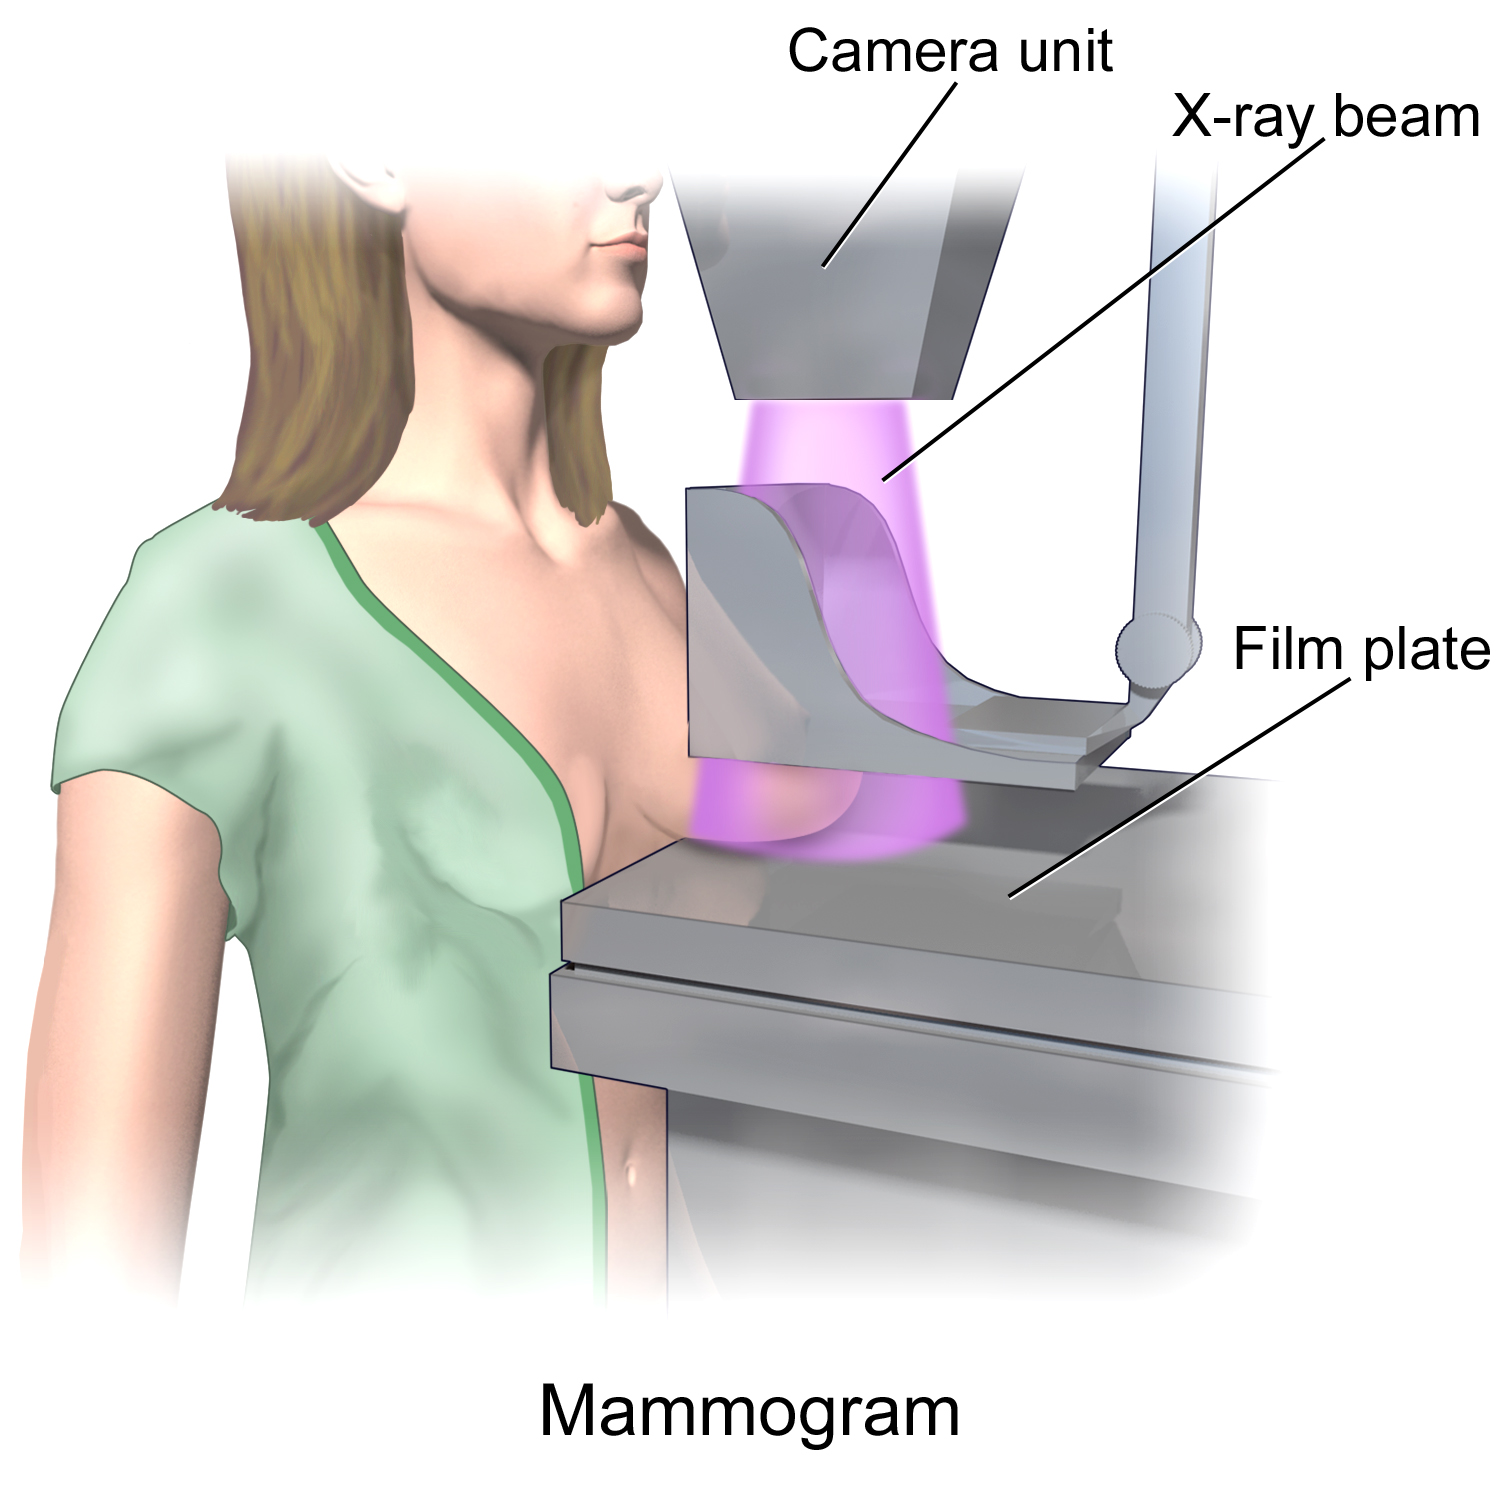
\includegraphics[height=9.65em]{Blausen_0628_Mammogram.png}}
~~~~~~~
{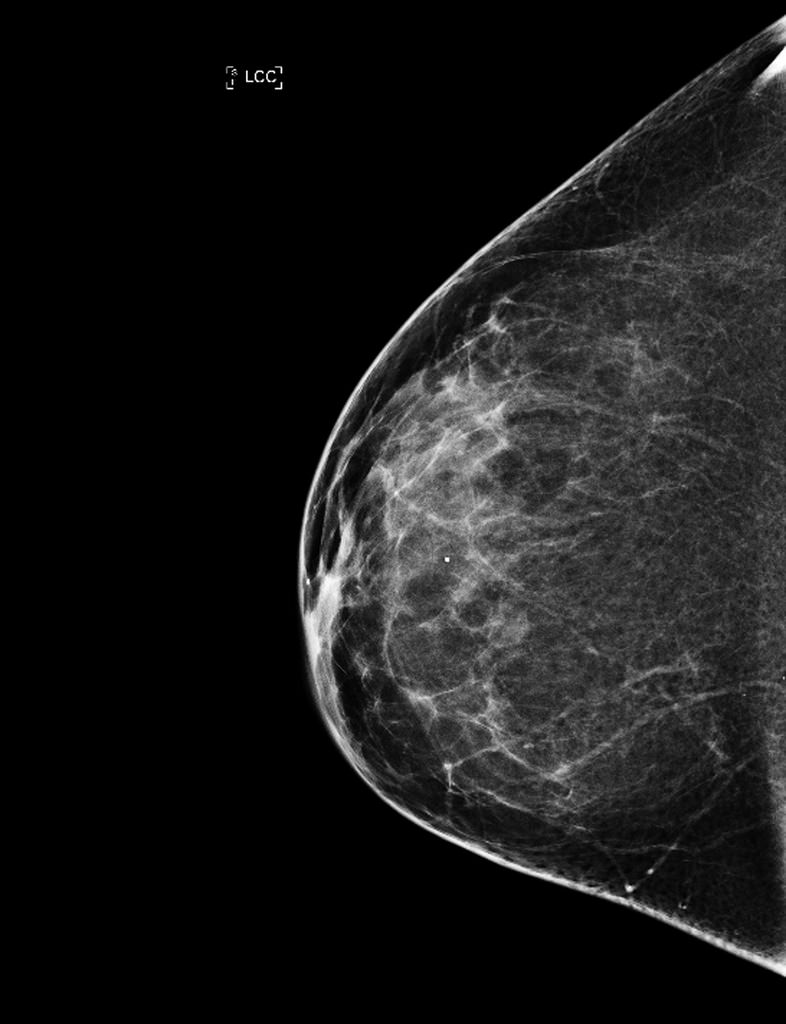
\includegraphics[height=9.65em]{mammography_exam.jpg}}
\vspace{0.34em} % When there are two boxes, some whitespace may need to be added if the one on the right has more content
\end{center}

}

%----------------------------------------------------------------------------------------
%	INTRODUCTION
%----------------------------------------------------------------------------------------

\headerbox{Introduction}{name=introduction,column=1,row=0,aligned=objectives}{
Rotation fill-in is a tumor sliding feature in ultrasound-elastography (UE) imaging modalities called Rotation Elastogram (RE) and Axial-Shear Strain Elastogram (ASSE) [1,2]. It comes from the bonding condition at the interface between the tumor and host tissue and may be used as a non-invasive breast-tumor classification tool (diagnosis) [1,2].\\
\\
This work aims to develop an automatic tumor-area detection method from Axial-Strain Elastogram (ASE) to estimate the rotation fill-in parameter during real-time UE scanning.
%\\The method aims to reducing the manual selection of lesion, which is operator dependent and cannot be used in real-time UE scanning.
}

%----------------------------------------------------------------------------------------
%	MATERIALS AND METHODS
%----------------------------------------------------------------------------------------

\headerbox{Rotation fill-in Method}{name=method,column=2,aligned=introduction}{ 
The automated rotation fill-in estimation method is based on morphological binary-image operations applied to ASE. The method consists in selecting the inside region of the inclusion (tumor model) in the ASSE image. \\
The size of different objects in the ASE binary image is reduced by using morphological operations generating its detaching. A size filter is then used to select the biggest area (tumor), which is then returned to its original size defining a tumor area filter. The latter is applied to the ASSE image to obtain the rotation fill-in parameter as:\\
\begin{center}
$ASSE_{fill-in}=\frac{|\overline{ASSE}|_{inside}}{|ASSE_{max}|.}$
\end{center}

This method is first tested using Finite-Element Analysis (FEA, ANSYS) and then validated using gelatin-glass-bead phantoms that mimic biological tissue.}

%----------------------------------------------------------------------------------------
%	EXPRIMENTAL SETUP
%----------------------------------------------------------------------------------------

\headerbox{FEA and In-vitro setup}{name=optimization,column=2,row=0,below=method }{
The 2D FEA simulations are performed following a multi-deformation scheme for isotropic elastic soft materials and the contact manager is used to emulate different bonding conditions of the inclusion (boundary conditions on the left figure).\\
\\
In-vitro validation is performed using an ultrasound linear-array probe (Terason 12L5-V) attached to compression device. The phantom is axially compressed in $\epsilon_0=1\%$ at different probe angles $\alpha$ and pre-compression levels (right figure).

\begin{center}
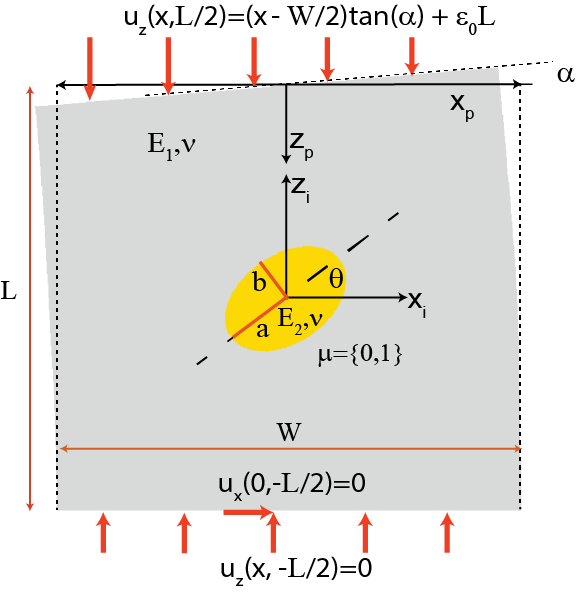
\includegraphics[height=9.6em]{Simus_setup.png}
~~~
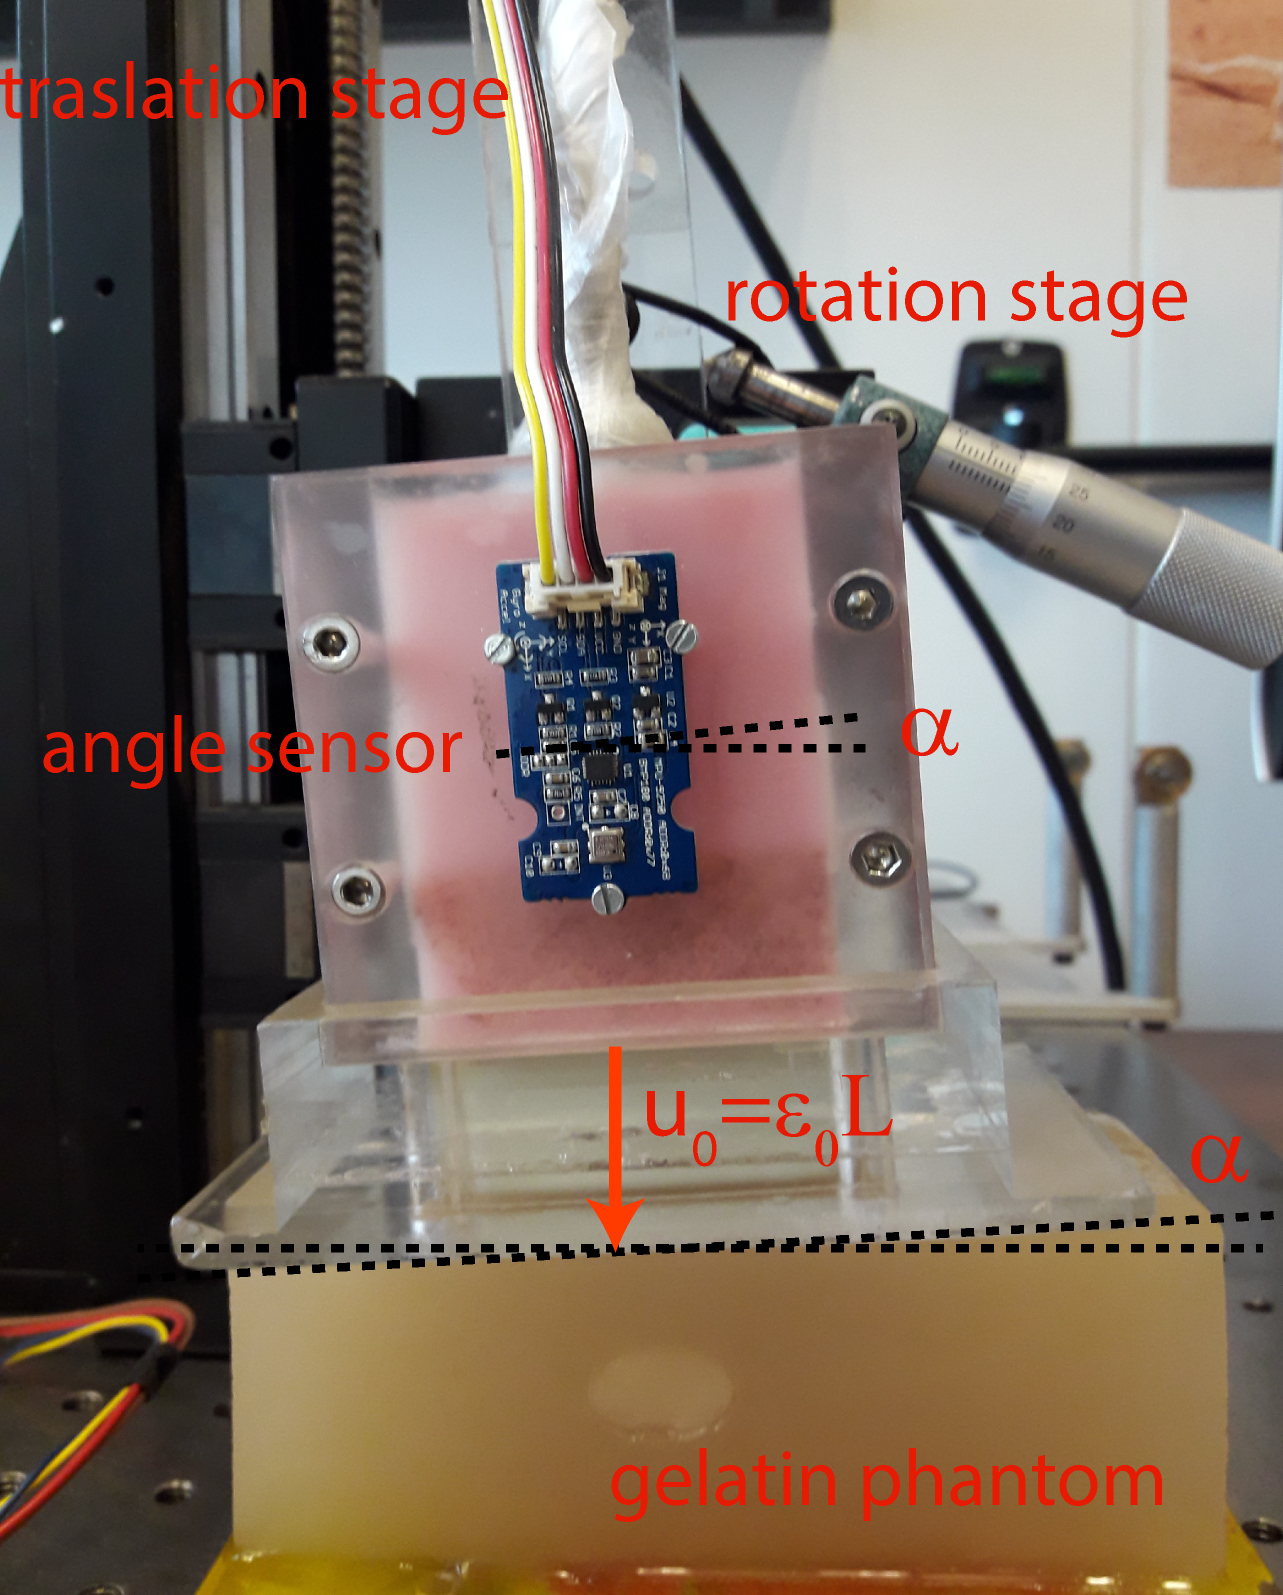
\includegraphics[height=10.74em]{Exp_setup.jpg}
\end{center}
\vspace{0.22em}
 }     

%----------------------------------------------------------------------------------------
%	CONCLUSION
%----------------------------------------------------------------------------------------

\headerbox{Conclusion}{name=conclusion,column=2,row=0,below=optimization}{
\begin{itemize}
\item{The proposed method for automated rotation fill-in estimation is validated by in-vitro experiments.}
\item{The method shows to be robust to elastographic images distortions introduced by the ultrasound probe angle.}

\end{itemize}
}     

%----------------------------------------------------------------------------------------
%	FUTURE RESEARCH
%----------------------------------------------------------------------------------------

\headerbox{Future Research}{name=futureresearch,column=2,below=conclusion}{ 
% This block is as tall as the references block 
% above=bottom
\begin{itemize}
\item{Further in-vivo studies will be necessary to fully validate this method.}
\item{Real-time implementation for in-vivo applications. \\}
\end{itemize}
}
%----------------------------------------------------------------------------------------
%	RESULTS 2
%----------------------------------------------------------------------------------------

\headerbox{Finite elements analysis results}{name=results2,column=0,span=2,below=introduction}{
\begin{multicols}{2}
\setlength{\columnsep}{1em}%
\begin{wrapfigure}{r}{0.2\textwidth}
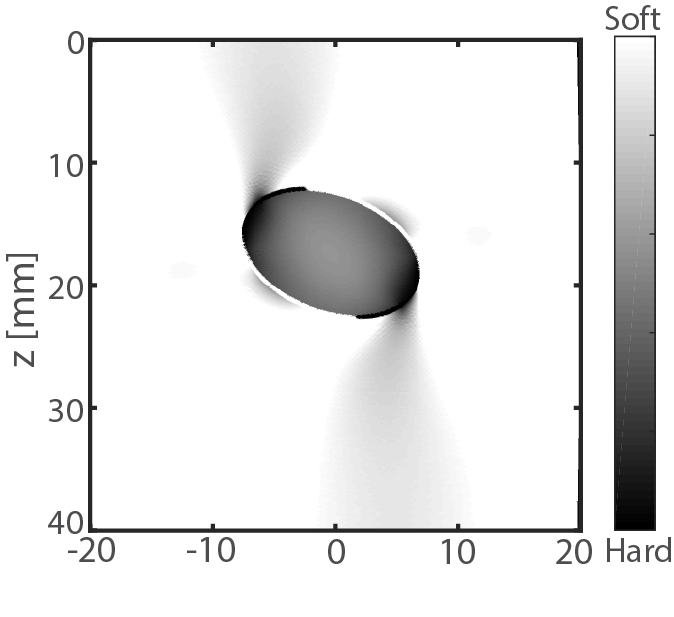
\includegraphics[height=9em]{Simus_filtering_fillin_orig.png}
\end{wrapfigure}

Top figures (left to right) show the computation of tumor-area filter (right) starting from the ASE image (left). The bottom figures show the corresponding application to ASSE image.
%Left figure shows pristine ASE image, the top figures show the computation of tumor area filter from the ASE image and the bottom figures the corresponding application to ASSE images. 

Simulations were performed for different ultrasound-probe angles ($\alpha$) and pre-compression levels to evaluate the robustness of the proposed method.

\begin{center}
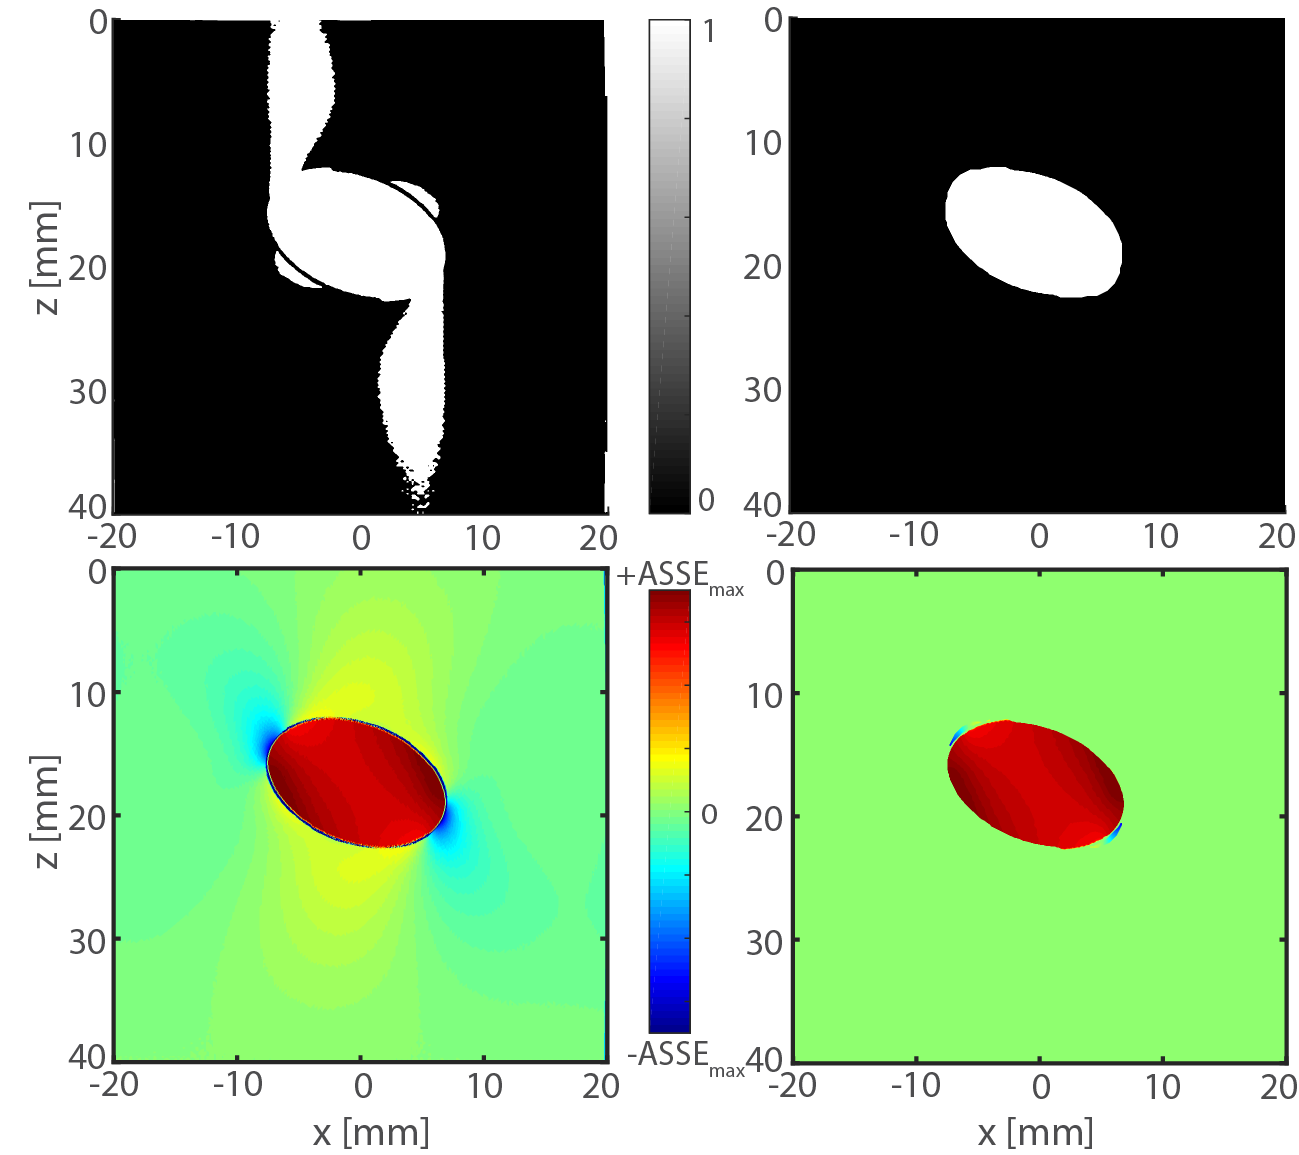
\includegraphics[height=17em]{Simus_filtering_fillin_v2.png}
\end{center}

\end{multicols}}

%----------------------------------------------------------------------------------------
%	RESULTS 2
%----------------------------------------------------------------------------------------

\headerbox{In-Vitro Validation}{name=results,column=0,span=2,row=0,aligned=results2,below=results2}{
\begin{multicols}{2}
 %Quasi-static ultrasound experiments are The ultrasound machine Terason T3000 Advanced controlled in Matlab ambiance is used to acquiring the rf-raw data in fashion in synchronism with the axial compression $\epsilon_0$ for each angle $\alpha$. The elastographic images (ASE and ASSE, Figure 2b-e) are obtained from rf-raw data using a multilevel 2D block-matching algorithm described in [3]. 
 
 \begin{center}
{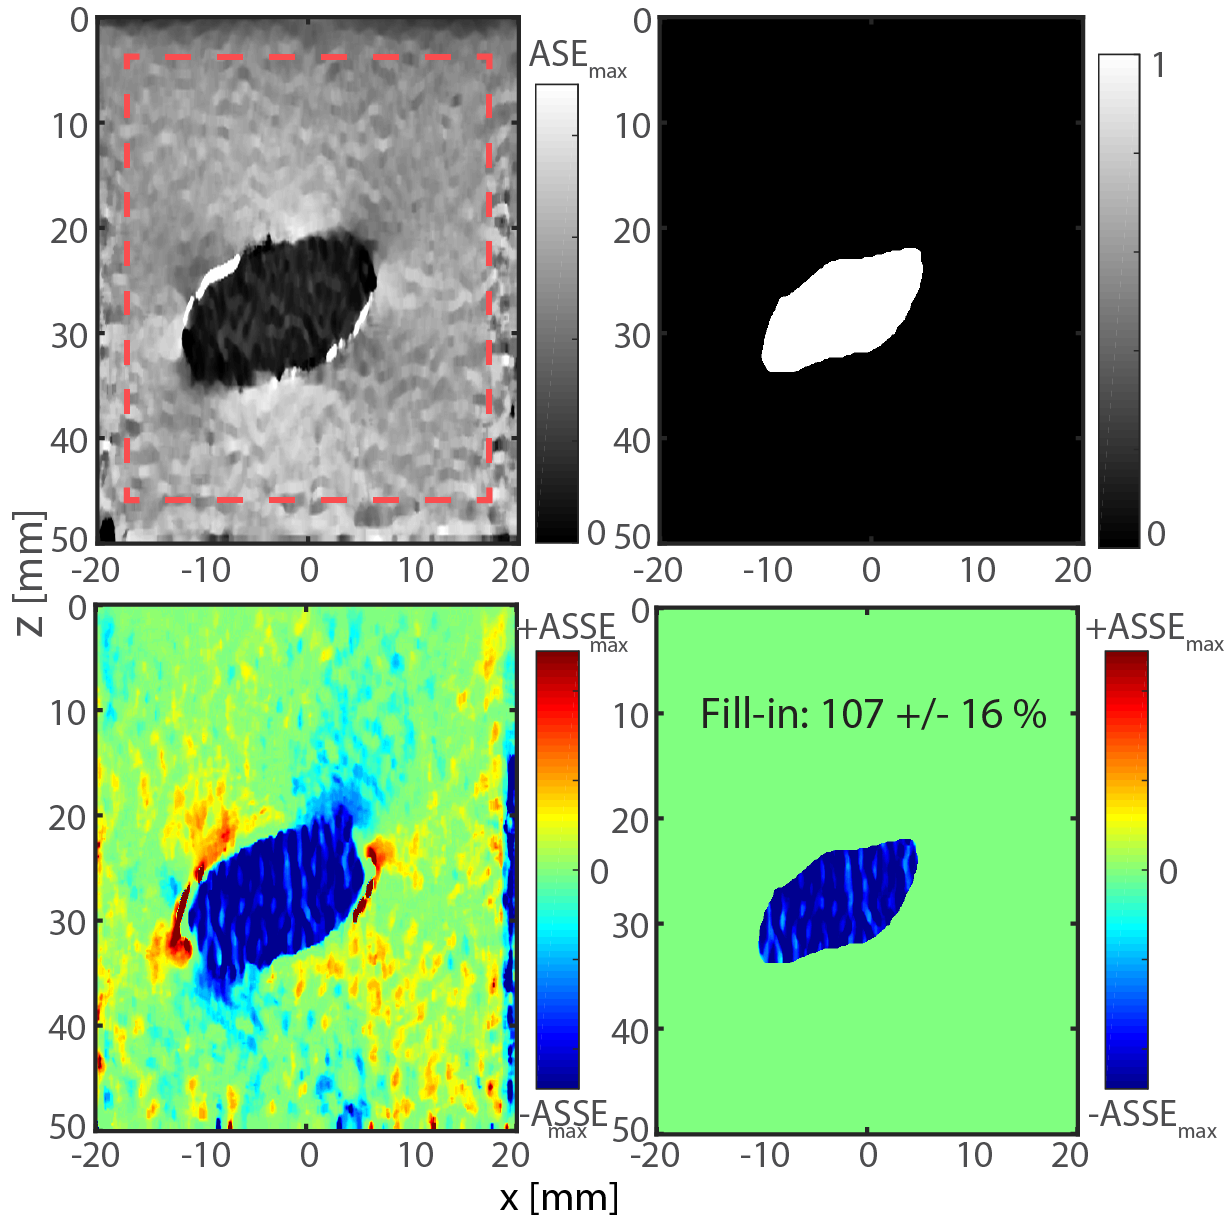
\includegraphics[height=20em]{ExpImages_v3.png}}
\end{center}
 The tumor-area filter calculation is shown on the top figures for a particular ASE image. This filter was applied to the entire cineloop of ASSE images and the rotation fill-in value was estimated. \\ 
 \\On bottom figure is shown the result for a loosely bounded inclusion ($\sim$100\%, see inset) without pre-compression for $\alpha=0$ (ideal case). \\
 %This results are consistent with previous studies [1,2].
 \\
 The method automatically selects the tumor area despite image noise. The results are consistent with previous studies [1,2].



\end{multicols}
}

%----------------------------------------------------------------------------------------
%	REFERENCES
%----------------------------------------------------------------------------------------

\headerbox{References}{name=references,column=0,below=results, above=bottom}{

\renewcommand{\section}[2]{\vskip 0.05em} % Get rid of the default "References" section title
\nocite{*} % Insert publications even if they are not cited in the poster
\small{ % Reduce the font size in this block
\bibliographystyle{unsrt}
\bibliography{references} % Use sample.bib as the bibliography file
}}


%----------------------------------------------------------------------------------------
%	CONTACT INFORMATION
%----------------------------------------------------------------------------------------

\headerbox{acknowledgements}{name=contact,column=1,below=results,above=bottom}{ 
% This block is as tall as the references block
This work is funded by the DICYT-Usach project No. 041731GD, Chile; "Fondo Concursable Facultad de Ciencia USACH 2018" and The Optical Society (OSA)\\

For more information please contact:
\begin{description}\compresslist
\item{-}belfor.galaz@usach.cl
\item{-}esteban.donoso@usach.cl
\end{description}
}


%----------------------------------------------------------------------------------------
\end{poster}
\end{document}